\chapter{DevOps}
In the old-style software engineering there are \textbf{separate} teams addressing software development, deployment, release and support.
The development team, or a separate maintenance team, is responsible for software updates and maintenance.\\
This approach introduces many issues, which can be summarized as \textbf{difficult communication} amongst teams, due to different tools, skills, etc. leading to requiring multiple to days to release an "urgent" patch.

\textit{Amazon} re-engineered its software into (micro)services assigning both service development and service support to the same team.

\section{Principles}

\labelitemize{\textbf{\textit{\underline{Principles}}}
}{
   \begin{enumerate}[label=\textbf{D\arabic*} - ,left=1em]
      \item \textit{Everyone is responsible for
      everything.}
      \begin{enumerate}
         \item 
         All team members have joint responsibility
         for developing, delivering, and supporting the
         software.
      \end{enumerate}
      \item \textit{Everything that can be automated
      should be automated}
      \begin{enumerate}
         \item 
         All activities involved in testing, deployment,
         and support should be automated if it is possible
         to do so. There should be mimimal manual
         involvement in deploying software.
      \end{enumerate}
      \item \textit{Measure first, change later}.
      \begin{enumerate}
         \item 
         DevOps should be driven by a measurement
         program where you collect data about the
         system and its operation. You then use the
         collected data to inform decisions about
         changing DevOps processes and tools.
      \end{enumerate}
   \end{enumerate}
}
\nl
\nl

\labelitemize{\textit{Benefits}}{
\begin{enumerate}
   \item \textit{Faster deployment}\\
   Software can be deployed to production more
   quickly because communication delays between
   the people involved in the process are dramatically
   reduced.
   \item \textit{Reduced risk}\\
   The increment of functionality in each release is
   small so there is less chance of feature interactions
   and other changes that cause system failures and
   outages.
   \item \textit{Faster repair}\\
   DevOps teams work together to get the software
   up and running again as soon as possible. There is
   no need to discover which team was responsible for
   the problem and to wait for them to fix it.
   \item \textit{More productive teams}\\
   DevOps teams are happier and more productive
   than the teams involved in the separate activities.
   Because team members are happier, they are less
   likely to leave to find jobs elsewhere.
\end{enumerate}
}

\section{Code Management}

\begin{figure}[htbp]
   \centering
   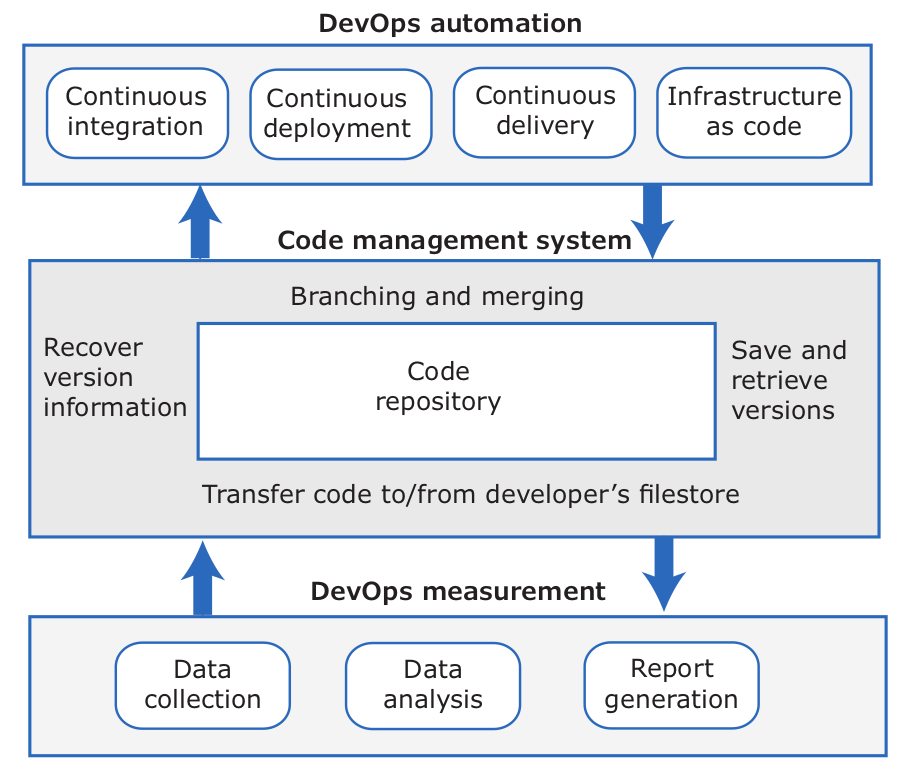
\includegraphics{images/codemanagement.png}
   \caption{Code management according to DevOps}
   \label{fig:codemanagement}
\end{figure}

Code must be \textbf{managed} using \texttt{git}, which is a \textit{decentralized system} which provides some crucial benefits:
\begin{enumerate}
   \item \textbf{Resilience}
   \begin{enumerate}
      \item Every dev has its \textit{own copy} of the project
      \item If the shared repository is damaged or subjected to a cyber-attack, work can continue and a previous state may be \textit{restored}
      \item Devs can \textit{work offline}
   \end{enumerate}
   \item \textbf{Speed}
   \begin{enumerate}
      \item Committing changes to the repository is a fast, \textit{local} operation
   \end{enumerate}
   \item \textbf{Flexibility}
   \begin{enumerate}
      \item Local experimentation is much simpler i.e. 
      Developers can safely try different approaches without exposing their experiments to other project members
   \end{enumerate}
\end{enumerate}

\section{Automation}

\textbf{Continuous integration} means that every time that a dev commits a change to project's main branch, 
an \textit{updated executable} version of the system is \textbf{built} and \textbf{tested}.

\textbf{Continuous delivery} refers to the testing environment, which must be the product's operating environment.

\textbf{Continuous deployment} means that every new release of the system should be seamlessy made available to users as soon as a change gets committed\footnote{Shouldn'it be tested first? \smiley} to the main branch.

\textbf{Infrastructure as Code}
Machine-readable models of the infrastructure \footnote{network, servers, routers, etc.} on which the product executes
are used by configuration management tools to build the
software’s execution platform. The software to be installed,
such as compilers and libraries and a DBMS, are included in the infastructure model.